\section{Secondary Analyses}
\label{app:secondary}

\subsection{Classification Results with Seed Variation}

\tableref{tab:classification-full} gives sample SDs for the capped probe and fine-tuning, and \tableref{tab:converged-probe} (Appendix~\ref{app:converged}) gives them for the converged probe. Figure~\ref{fig:seed-differences} shows matched-seed paired differences, \MAE{} minus each comparator.

\begin{table*}[htbp]
\floatconts
  {tab:classification-full}
  {\caption{Core classification AUPRC, mean (sample SD) over five matched seeds. Probe rows use the capped linear probe. Bold marks the highest unrounded mean in each row. The supervised Transformer is defined only for full fine-tuning.}}
  {\scriptsize
  \begin{tabular}{lllrrrr}
\toprule
Data & Protocol & Endpoint & MAE & JEPA & Contrastive & Supervised \\
\midrule
Combined & Fine-tune & 24h mortality & \textbf{0.409 (0.024)} & 0.391 (0.031) & 0.399 (0.029) & 0.389 (0.021) \\
Combined & Fine-tune & Hospital mortality & \textbf{0.531 (0.010)} & 0.521 (0.009) & 0.514 (0.016) & 0.518 (0.008) \\
Combined & Fine-tune & AKI & 0.626 (0.004) & 0.626 (0.005) & 0.614 (0.004) & \textbf{0.652 (0.003)} \\
Combined & Probe & 24h mortality & \textbf{0.284 (0.031)} & 0.188 (0.018) & 0.205 (0.016) & -- \\
Combined & Probe & Hospital mortality & \textbf{0.470 (0.013)} & 0.357 (0.006) & 0.392 (0.010) & -- \\
Combined & Probe & AKI & \textbf{0.447 (0.006)} & 0.327 (0.005) & 0.396 (0.005) & -- \\
eICU-CRD & Fine-tune & 24h mortality & \textbf{0.377 (0.013)} & 0.363 (0.008) & 0.360 (0.016) & 0.351 (0.022) \\
eICU-CRD & Fine-tune & Hospital mortality & \textbf{0.495 (0.005)} & 0.471 (0.007) & 0.471 (0.003) & 0.474 (0.004) \\
eICU-CRD & Fine-tune & AKI & 0.519 (0.017) & 0.515 (0.018) & 0.494 (0.012) & \textbf{0.554 (0.014)} \\
eICU-CRD & Probe & 24h mortality & \textbf{0.276 (0.015)} & 0.199 (0.017) & 0.195 (0.009) & -- \\
eICU-CRD & Probe & Hospital mortality & \textbf{0.439 (0.006)} & 0.355 (0.004) & 0.350 (0.010) & -- \\
eICU-CRD & Probe & AKI & \textbf{0.361 (0.009)} & 0.268 (0.008) & 0.286 (0.004) & -- \\
MIMIC-IV & Fine-tune & 24h mortality & 0.451 (0.045) & 0.451 (0.050) & \textbf{0.456 (0.042)} & 0.449 (0.032) \\
MIMIC-IV & Fine-tune & Hospital mortality & \textbf{0.579 (0.011)} & 0.564 (0.009) & 0.568 (0.011) & 0.565 (0.008) \\
MIMIC-IV & Fine-tune & AKI & 0.667 (0.009) & 0.642 (0.009) & 0.645 (0.009) & \textbf{0.693 (0.013)} \\
MIMIC-IV & Probe & 24h mortality & \textbf{0.312 (0.042)} & 0.236 (0.028) & 0.254 (0.035) & -- \\
MIMIC-IV & Probe & Hospital mortality & \textbf{0.510 (0.014)} & 0.415 (0.020) & 0.458 (0.023) & -- \\
MIMIC-IV & Probe & AKI & \textbf{0.504 (0.009)} & 0.410 (0.017) & 0.478 (0.009) & -- \\
\bottomrule
\end{tabular}
}
\end{table*}

\begin{figure*}[htbp]
\floatconts
  {fig:seed-differences}
  {\caption{Matched-seed classification AUPRC differences, MAE minus comparator. Positive values favor MAE. Points are mean paired differences. Bars span the five observed differences, not a confidence interval. Supervised appears only for full fine-tuning.}}
  {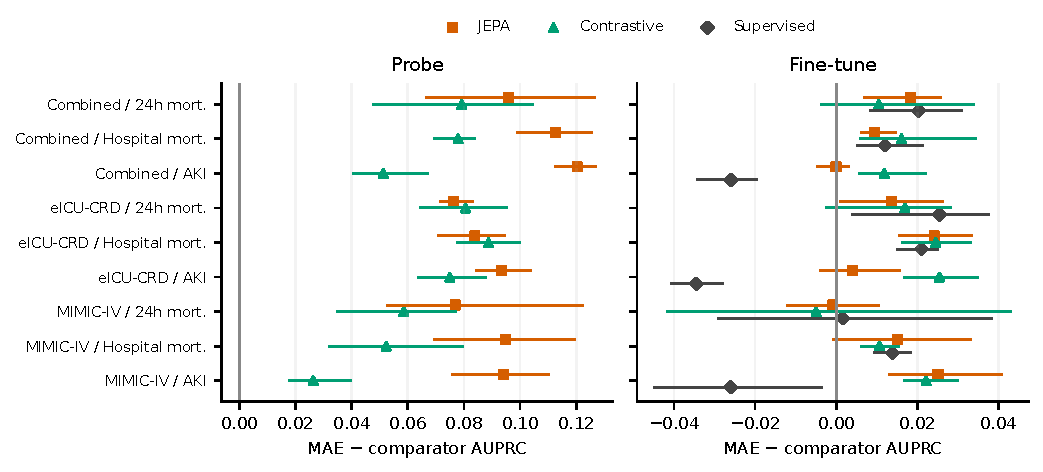
\includegraphics[width=.92\textwidth]{generated/seed-variance.pdf}}
\end{figure*}

\subsection{Label Efficiency}
\label{app:label-efficiency}

\begin{figure*}[htbp]
\floatconts
  {fig:label-efficiency}
  {\caption{Hospital-mortality label efficiency under full fine-tuning, including the supervised Transformer at each label fraction. Points are five-seed means. Bars are sample SD across seeds. Only training labels are reduced.}}
  {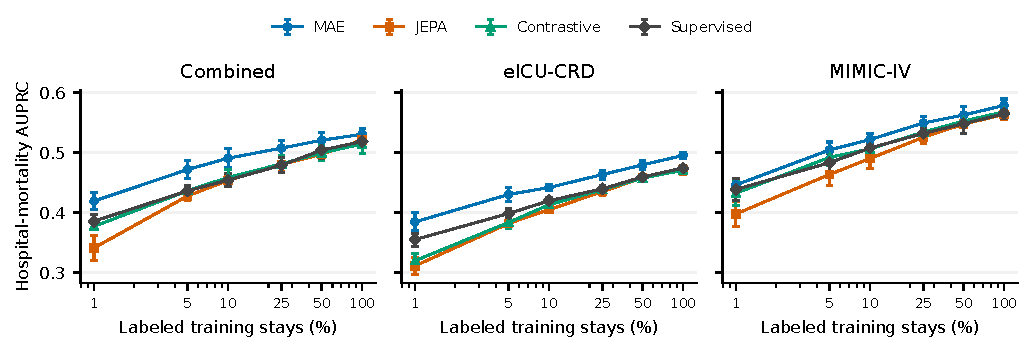
\includegraphics[width=.94\textwidth]{generated/label-efficiency.pdf}}
\end{figure*}

Only the labeled training subset is reduced. Validation and test partitions remain unchanged. Each seed draws its subsets as prefixes of one random permutation of the labeled training stays, keeping $\lfloor fn \rfloor$ of $n$ stays at fraction $f$. Subsets are therefore nested across fractions within a seed and are not class-stratified. Hospital mortality uses 1\%, 5\%, 10\%, 25\%, 50\%, and the full-label reference. Twenty-four-hour mortality starts at 5\%. AKI and LOS use 10\% and full-label references. Each cell contains five seeds.


At the lowest exported fraction for \Combined{} hospital mortality (1\%), fine-tuned AUPRC means are .419 for \MAE{}, .341 for \JEPA{}, .377 for contrastive learning, and .386 for supervised training. At 5\% labels for 24-hour mortality, the corresponding means are .277, .241, .245, and .267. When full-label references are included, MAE leads 39/45 fine-tuning cells among SSL methods, 35/45 with supervised included, and 37/39 classification probe cells among SSL methods (LOS probe cells use the superseded capped probe). Section~\ref{sec:results} instead counts only fractions below 100\%. Comparator sets and denominators must be stated together.

\begin{table*}[htbp]
\floatconts{tab:low-label}{\caption{Lowest exported label fractions, full fine-tuning. MAE and supervised means use AUPRC for classification and absolute error in days for LOS. $\Delta$ is MAE minus supervised. Positive favors MAE only for classification. SD is computed from five paired differences, not from independent error propagation.}}
{\scriptsize\begin{tabular}{lllrrrr}
\toprule
Data & Task & Labels & MAE & Supervised & $\Delta$ mean & $\Delta$ SD \\
\midrule
Combined & 24h mortality & 5\% & 0.277 & 0.267 & 0.010 & 0.027 \\
Combined & Hospital mortality & 1\% & 0.419 & 0.386 & 0.033 & 0.012 \\
Combined & AKI & 10\% & 0.514 & 0.507 & 0.006 & 0.021 \\
Combined & Remaining LOS & 10\% & 2.229 & 2.252 & -0.023 & 0.024 \\
eICU-CRD & 24h mortality & 5\% & 0.260 & 0.248 & 0.011 & 0.015 \\
eICU-CRD & Hospital mortality & 1\% & 0.385 & 0.355 & 0.029 & 0.019 \\
eICU-CRD & AKI & 10\% & 0.405 & 0.411 & -0.006 & 0.009 \\
eICU-CRD & Remaining LOS & 10\% & 2.067 & 2.081 & -0.014 & 0.034 \\
MIMIC-IV & 24h mortality & 5\% & 0.294 & 0.268 & 0.026 & 0.041 \\
MIMIC-IV & Hospital mortality & 1\% & 0.446 & 0.439 & 0.008 & 0.021 \\
MIMIC-IV & AKI & 10\% & 0.565 & 0.549 & 0.016 & 0.012 \\
MIMIC-IV & Remaining LOS & 10\% & 2.494 & 2.490 & 0.004 & 0.071 \\
\bottomrule
\end{tabular}
}
\end{table*}

Figure~\ref{fig:label-efficiency} shows hospital mortality. \tableref{tab:label-fraction-delta} extends the comparison to every label fraction. For hospital mortality, fine-tuned \MAE{} exceeds supervised training at every fraction in every regime. The difference is largest at low fractions on \Combined{} and \EICU{} and does not vanish at full labels. For 24-hour mortality it is also positive at every fraction on \EICU{} and \Combined{}. On \MIMIC{}, the smallest cohort, the 24-hour-mortality differences above 5\% labels change sign. For AKI, supervised training leads at full labels in all three regimes. The answer to when pretraining stops paying off therefore depends on endpoint and cohort more than on the label fraction.

Because subsets are drawn without class stratification, their positive counts vary by seed (\tableref{tab:low-label-positives}). The counts were recomputed after review from the same split and subset rules. The same rules reproduce the exported test support exactly. \MIMIC{} 24-hour mortality at 5\% labels has 31--43 training positives and also the largest AUPRC paired-difference SD in \tableref{tab:low-label}.

\begin{table*}[htbp]
\floatconts{tab:label-fraction-delta}{\caption{Mean paired difference between fine-tuned \MAE{} and the supervised Transformer at each label fraction, five seeds. Classification uses AUPRC, where positive favors \MAE{}. LOS uses absolute error in days, where negative favors \MAE{}. Dashes mark fractions that were not run.}}
{\scriptsize\begin{tabular}{llrrrrrr}
\toprule
Data & Task & 1\% & 5\% & 10\% & 25\% & 50\% & 100\% \\
\midrule
Combined & 24h mortality & -- & 0.010 & 0.021 & 0.033 & 0.020 & 0.020 \\
Combined & Hospital mortality & 0.033 & 0.036 & 0.036 & 0.028 & 0.016 & 0.012 \\
Combined & AKI & -- & -- & 0.006 & -- & -- & -0.026 \\
Combined & Remaining LOS & -- & -- & -0.023 & -- & -- & -0.072 \\
eICU-CRD & 24h mortality & -- & 0.011 & 0.010 & 0.026 & 0.035 & 0.026 \\
eICU-CRD & Hospital mortality & 0.029 & 0.032 & 0.022 & 0.024 & 0.020 & 0.021 \\
eICU-CRD & AKI & -- & -- & -0.006 & -- & -- & -0.034 \\
eICU-CRD & Remaining LOS & -- & -- & -0.014 & -- & -- & -0.032 \\
MIMIC-IV & 24h mortality & -- & 0.026 & -0.020 & -0.016 & -0.008 & 0.002 \\
MIMIC-IV & Hospital mortality & 0.008 & 0.021 & 0.014 & 0.017 & 0.015 & 0.014 \\
MIMIC-IV & AKI & -- & -- & 0.016 & -- & -- & -0.026 \\
MIMIC-IV & Remaining LOS & -- & -- & 0.004 & -- & -- & -0.029 \\
\bottomrule
\end{tabular}
}
\end{table*}

\begin{table*}[htbp]
\floatconts{tab:low-label-positives}{\caption{Positive training labels in each reduced-label subset, by seed, with the mean number of labeled training stays. Only the labeled training subset is reduced. Subsets are drawn per seed without class stratification. Counts were recomputed after review.}}
{\scriptsize\begin{tabular}{lllrrrrrrr}
\toprule
 & & & \multicolumn{6}{c}{Labeled training positives} & \\
\cmidrule(lr){4-9}
Data & Task & Labels & 42 & 123 & 456 & 789 & 1011 & Mean & Labeled stays \\
\midrule
Combined & 24h mortality & 5\% & 144 & 117 & 110 & 118 & 116 & 121.0 & 7,214.0 \\
Combined & 24h mortality & 10\% & 263 & 241 & 219 & 218 & 236 & 235.4 & 14,428.6 \\
Combined & 24h mortality & 25\% & 594 & 605 & 580 & 560 & 586 & 585.0 & 36,072.2 \\
Combined & 24h mortality & 50\% & 1,124 & 1,197 & 1,143 & 1,131 & 1,139 & 1,146.8 & 72,144.4 \\
Combined & Hospital mortality & 1\% & 144 & 164 & 150 & 159 & 150 & 153.4 & 1,442.6 \\
Combined & Hospital mortality & 5\% & 704 & 765 & 756 & 737 & 701 & 732.6 & 7,215.6 \\
Combined & Hospital mortality & 10\% & 1,427 & 1,457 & 1,489 & 1,511 & 1,444 & 1,465.6 & 14,431.8 \\
Combined & Hospital mortality & 25\% & 3,635 & 3,687 & 3,641 & 3,766 & 3,622 & 3,670.2 & 36,080.0 \\
Combined & Hospital mortality & 50\% & 7,236 & 7,366 & 7,363 & 7,508 & 7,304 & 7,355.4 & 72,160.4 \\
Combined & AKI & 10\% & 1,625 & 1,656 & 1,600 & 1,685 & 1,724 & 1,658.0 & 10,126.6 \\
eICU-CRD & 24h mortality & 5\% & 69 & 57 & 61 & 68 & 71 & 65.2 & 4,600.6 \\
eICU-CRD & 24h mortality & 10\% & 139 & 140 & 143 & 125 & 137 & 136.8 & 9,201.8 \\
eICU-CRD & 24h mortality & 25\% & 387 & 367 & 380 & 357 & 365 & 371.2 & 23,005.2 \\
eICU-CRD & 24h mortality & 50\% & 768 & 746 & 722 & 751 & 700 & 737.4 & 46,011.2 \\
eICU-CRD & Hospital mortality & 1\% & 80 & 85 & 95 & 78 & 74 & 82.4 & 919.8 \\
eICU-CRD & Hospital mortality & 5\% & 434 & 433 & 424 & 388 & 412 & 418.2 & 4,600.6 \\
eICU-CRD & Hospital mortality & 10\% & 840 & 888 & 892 & 797 & 827 & 848.8 & 9,201.8 \\
eICU-CRD & Hospital mortality & 25\% & 1,987 & 2,145 & 2,153 & 2,069 & 2,081 & 2,087.0 & 23,005.2 \\
eICU-CRD & Hospital mortality & 50\% & 4,137 & 4,234 & 4,233 & 4,217 & 4,143 & 4,192.8 & 46,011.2 \\
eICU-CRD & AKI & 10\% & 849 & 818 & 837 & 852 & 837 & 838.6 & 6,171.4 \\
MIMIC-IV & 24h mortality & 5\% & 31 & 34 & 43 & 40 & 37 & 37.0 & 2,608.6 \\
MIMIC-IV & 24h mortality & 10\% & 76 & 79 & 72 & 86 & 85 & 79.6 & 5,217.4 \\
MIMIC-IV & 24h mortality & 25\% & 216 & 199 & 190 & 207 & 202 & 202.8 & 13,044.2 \\
MIMIC-IV & 24h mortality & 50\% & 433 & 386 & 396 & 417 & 425 & 411.4 & 26,088.8 \\
MIMIC-IV & Hospital mortality & 1\% & 61 & 56 & 69 & 68 & 74 & 65.6 & 521.8 \\
MIMIC-IV & Hospital mortality & 5\% & 292 & 297 & 307 & 311 & 293 & 300.0 & 2,609.8 \\
MIMIC-IV & Hospital mortality & 10\% & 633 & 608 & 624 & 610 & 608 & 616.6 & 5,220.2 \\
MIMIC-IV & Hospital mortality & 25\% & 1,582 & 1,532 & 1,548 & 1,522 & 1,463 & 1,529.4 & 13,052.0 \\
MIMIC-IV & Hospital mortality & 50\% & 3,102 & 3,116 & 3,090 & 3,029 & 3,020 & 3,071.4 & 26,104.4 \\
MIMIC-IV & AKI & 10\% & 787 & 804 & 785 & 819 & 761 & 791.2 & 3,951.6 \\
\bottomrule
\end{tabular}
}
\end{table*}

\subsection{Cross-Database Adaptation}
\label{app:transfer}

Cross-database rows pretrain on one database and then fully fine-tune using labels from the other. They test whether a representation pretrained under one site's measurement practice can be adapted with target labels. They are not out-of-domain validation: no model is evaluated on a database without training on its labels. MAE has the best mean primary metric on three of four \MIMIC{}-to-\EICU{} tasks and ties contrastive learning on the fourth, AKI (.532 each). It leads three of four reverse-direction tasks, and contrastive learning leads reverse-direction 24-hour mortality (\tableref{tab:transfer}).

\tableref{tab:transfer-context} places cross-database \MAE{} beside \MAE{} pretrained on the target database and the supervised Transformer trained on the target. These comparators come from the core comparison with matched seeds. For mortality, cross-database encoders stay within .004--.010 AUPRC of target-database pretraining. For AKI, supervised training leads regardless of pretraining source. These are five-seed means, not tests of equivalence, and do not establish a general transfer advantage.

\begin{table*}[htbp]
\floatconts
  {tab:transfer}
  {\caption{Cross-database full-fine-tuning means over five seeds. Classification uses AUPRC. LOS uses absolute error in days. Bold marks the best mean within each row, and every mean that ties it at three decimals.}}
  {\scriptsize
  \begin{tabular}{llllrrr}
\toprule
Pretrain & Target & Task & Metric & MAE & JEPA & Contrastive \\
\midrule
eICU-CRD & MIMIC-IV & 24h mortality & AUPRC & 0.447 & 0.453 & \textbf{0.454} \\
eICU-CRD & MIMIC-IV & Hospital mortality & AUPRC & \textbf{0.572} & 0.559 & 0.564 \\
eICU-CRD & MIMIC-IV & AKI & AUPRC & \textbf{0.646} & 0.643 & 0.627 \\
eICU-CRD & MIMIC-IV & Remaining LOS & Abs. error & \textbf{2.389} & 2.390 & 2.403 \\
MIMIC-IV & eICU-CRD & 24h mortality & AUPRC & \textbf{0.372} & 0.367 & 0.354 \\
MIMIC-IV & eICU-CRD & Hospital mortality & AUPRC & \textbf{0.485} & 0.477 & 0.476 \\
MIMIC-IV & eICU-CRD & AKI & AUPRC & \textbf{0.532} & 0.520 & \textbf{0.532} \\
MIMIC-IV & eICU-CRD & Remaining LOS & Abs. error & \textbf{1.966} & 1.987 & 1.998 \\
\bottomrule
\end{tabular}
}
\end{table*}

\begin{table*}[htbp]
\floatconts
  {tab:transfer-context}
  {\caption{Fine-tuned \MAE{} on each target database, by pretraining source, beside the supervised Transformer trained from scratch on the target. Means over five seeds. Classification uses AUPRC. LOS uses absolute error in days. Bold marks the best mean in each row.}}
  {\scriptsize
  \begin{tabular}{lllrrr}
\toprule
Target & Task & Metric & Other-DB pretraining & Target-DB pretraining & Supervised \\
\midrule
eICU-CRD & 24h mortality & AUPRC & 0.372 & \textbf{0.377} & 0.351 \\
eICU-CRD & Hospital mortality & AUPRC & 0.485 & \textbf{0.495} & 0.474 \\
eICU-CRD & AKI & AUPRC & 0.532 & 0.519 & \textbf{0.554} \\
eICU-CRD & Remaining LOS & Abs. error & 1.966 & \textbf{1.964} & 1.997 \\
MIMIC-IV & 24h mortality & AUPRC & 0.447 & \textbf{0.451} & 0.449 \\
MIMIC-IV & Hospital mortality & AUPRC & 0.572 & \textbf{0.579} & 0.565 \\
MIMIC-IV & AKI & AUPRC & 0.646 & 0.667 & \textbf{0.693} \\
MIMIC-IV & Remaining LOS & Abs. error & 2.389 & \textbf{2.368} & 2.397 \\
\bottomrule
\end{tabular}
}
\end{table*}

\subsection{Encoder Capacity and Subgroup Auditing}
\label{app:capacity-subgroups}

The capacity analysis compares MAE and supervised Transformers on \MIMIC{} 24-hour mortality at 5\%, 10\%, and 50\% labels. Under full fine-tuning, medium and large MAE models exceed their corresponding supervised models by .013--.028 mean AUPRC across the six size--fraction cells, each with five seeds. This one-task, one-database slice does not test larger JEPA or contrastive encoders and cannot establish a general scaling rule.

Subgroup auditing records maximum-minus-minimum performance gaps across eligible gender, age, and race groups, requiring at least 50 unique patients and a defined metric per group. In the core full-label classification cells, across-seed mean AUPRC gaps range from .004 to .095 for gender, .033 to .172 for age, and .080 to .513 for race. These ranges cover 63 gender cells, 63 age cells, and 42 race cells. Race metrics are unavailable for \EICU{}, and \Combined{} race analyses use \MIMIC{}-origin records. A 50-patient threshold does not ensure enough positive outcomes for stable AUPRC. These summaries describe gaps without ranking methods by fairness or attributing their causes. They do not assess intersectional groups or subgroup calibration.

\subsection{TS2Vec Context}

\label{app:ts2vec}

Our TS2Vec-style extension retains the SLICES Transformer and value--mask interface, rather than the original dilated convolutional encoder. It adds Gaussian noise of SD .01 to observed values, independently masks half the hours in each view, and uses no temporal crop in the reference configuration. A width-256/output-64 projection precedes temperature-.05 NT-Xent over overlapping timestep pairs. Negatives combine other times and other instances in one denominator. This differs from original TS2Vec's separate temporal and instance losses. Four max-pooling scales (1, 2, 4, 8 hours) use mask-aware validity and an average over active scales. Thus these results characterize this extension, not original TS2Vec's performance \citep{yue2022ts2vec}.

\begin{table*}[htbp]
\floatconts
  {tab:ts2vec}
  {\caption{TS2Vec-style extension versus the core contrastive implementation. Entries count dataset--task cells with the better unrounded mean among 12 cells per protocol.}}
  {\begin{tabular}{lrr}
\toprule
Protocol & TS2Vec-style & Core contrastive \\
\midrule
Fine-tune & 8 & 4 \\
Probe & 0 & 12 \\
\bottomrule
\end{tabular}
}
\end{table*}

\tableref{tab:ts2vec} counts the cells each implementation wins. The full-fine-tuning split is task dependent. For example, TS2Vec is higher on \MIMIC{} 24-hour mortality (.465 versus .456), while core contrastive is lower on \MIMIC{} LOS (2.359 versus 2.370). Under the capped probe, the core contrastive mean is better in every cell, including \MIMIC{} AKI (.478 versus .441) and LOS (2.592 versus 2.722). The TS2Vec-style encoders were not refit with converged or loss-matched probes. These five-seed differences do not establish equivalence or general dominance.
